\subsection{A transitivity property}

Let X be a locally compact space in which a locally compact group H acts on the right, continuously and properly, by \((x,\xi)\mapsto x\xi\) \((x\in\mathbf{X},\xi\in\mathbf{H})\) . Let \(H'\) be a closed subgroup of H; then \(H'\) operates on the right in X, continuously and properly. We shall denote by \(\pi,\pi',p\) the canonical mappings of X onto X/H, of X onto \(X/H'\) , and of H onto \(H/H'\) .

Let \(\beta, \beta'\) be left Haar measures on H, H'; suppose that \(\Delta_{\mathrm{H}}\) and \(\Delta_{\mathrm{H}'}\) coincide on H'; one can then form the measure \(\beta / \beta'\) on H/H', left-invariant under H (No.~6, Th. 3). On the other hand, let \(\mu\) be a positive measure on X such that

\[
\delta (\xi) \mu = \Delta_ {\mathrm{H}} (\xi) \mu
\]

for \(\xi \in \mathbf{H}\) ; one can then form the measures \(\mu / \beta\) on \(\mathrm{X} / \mathrm{H}\) and \(\mu / \beta'\) on \(\mathrm{X} / \mathrm{H}'\) (No.~2, Prop. 4). We are going to write \(\mu / \beta'\) as the integral, with respect to \(\mu / \beta\) , of a family of measures on \(\mathrm{X} / \mathrm{H}'\) indexed by the points of \(\mathrm{X} / \mathrm{H}\) . When \(\mathrm{H}' = \{e\}\) , we shall find ourselves again in the situation of No.~3.

\pandocbounded{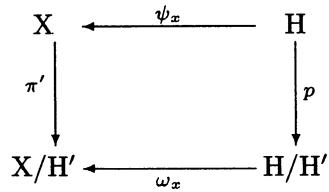
\includegraphics[keepaspectratio]{images/part001_c0ba5876.jpg}}

The mapping \((x,\xi)\mapsto\pi'(x\xi)\) of \(X\times H\) into \(X/H'\) is continuous; since \(\pi'(x\xi)=\pi'(x\xi\xi')\) for all \(\xi'\in H'\) this mapping defines, by passage to the quotient, a continuous mapping of \(X\times(H/H')\) into \(X/H'\) ; whence, for each fixed x in X, a partial mapping \(\omega_{x}\) of \(H/H'\) into \(X/H'\) , deduced by passage to the quotient from the mapping \(\psi_x: \xi \mapsto x\xi\) of H into X. Note that \(\psi_{x\xi} = \psi_x \circ \gamma_H(\xi)\) , therefore that \(\omega_{x\xi} = \omega_x \circ \gamma_{\mathrm{H/H'}}(\xi)\) for all \(\xi \in \mathrm{H}\) .

Lemma 7. --- Let K be a compact subset of X/H', and L a compact subset of X. Then \(\bigcup_{x\in\mathbf{L}}\omega_{x}^{-1}(\mathbf{K})\) is relatively compact in H/H'.

Let \(\mathbf{K}_1\) be a compact subset of \(\mathbf{X}\) such that \(\pi'(\mathbf{K}_1) = \mathbf{K}\) . Let \(\mathbf{K}_2\) be the set of \(\xi \in \mathbf{H}\) such that \(\mathbf{L}\xi\) intersects \(\mathbf{K}_1\) . Then \(\mathbf{K}_2\) is compact (GT, III, §4, No.~5, Th. 1). Let \(\xi \in \mathbf{H}\) be such that \(p(\xi) \in \bigcup_{x \in \mathbf{L}} \omega_x^{-1}(\mathbf{K})\) . Thus, there exists an \(x \in \mathbf{L}\) such that \(\omega_x(p(\xi)) \in \mathbf{K}\) , in other words such that \(\pi'(x\xi) \in \mathbf{K}\) . Since \(\pi'(\mathbf{K}_1) = \mathbf{K}\) , there exists \(\xi' \in \mathbf{H}'\) such that \(x\xi\xi' \in \mathbf{K}_1\) . Then \(\xi\xi' \in \mathbf{K}_2\) , therefore \(p(\xi) = p(\xi\xi') \in p(\mathbf{K}_2)\) . We have thus shown that \(\bigcup_{x \in \mathbf{L}} \omega_x^{-1}(\mathbf{K}) \subset p(\mathbf{K}_2)\) .

This lemma shows first of all that the mapping \(\omega_x\) is proper. One can therefore form the measure \(\omega_x(\beta/\beta')\) on \(\mathbf{X}/\mathbf{H}'\) , which is concentrated on \(\omega_x(\mathbf{H}/\mathbf{H}') = \pi'(\psi_x(\mathbf{H})) = \pi'(x\mathbf{H})\) . If \(f \in \mathcal{K}(\mathbf{X}/\mathbf{H}')\) , Lemma 7 and §1, No.~1, Lemma 1 show that the function \(x \mapsto \langle f, \omega_x(\beta/\beta') \rangle\) is continuous on \(\mathbf{X}\) ; moreover, \(\langle f, \omega_x(\beta/\beta') \rangle\) is zero when \(\operatorname{Supp} f\) does not intersect \(\pi'(x\mathbf{H})\) , in other words when \(\pi(x)\) does not belong to the canonical image of \(\operatorname{Supp} f\) in \(\mathbf{X}/\mathbf{H}\) .

Moreover, if \(x \in H\) then

\[
\omega_ {x \xi} (\beta / \beta^ {\prime}) = \omega_ {x} \left(\boldsymbol {\gamma} _ {\mathrm{H} / \mathrm{H} ^ {\prime}} (\xi) (\beta / \beta^ {\prime})\right) = \omega_ {x} (\beta / \beta^ {\prime}).
\]

The mapping \(x \mapsto \omega_x(\beta/\beta')\) of X into \(\mathcal{M}(\mathrm{X}/\mathrm{H}')\) therefore defines by passage to the quotient a mapping \(u \mapsto (\beta/\beta')_u\) of X/H into \(\mathcal{M}(\mathrm{X}/\mathrm{H}')\) . The foregoing shows that, for every \(f \in \mathcal{K}(\mathrm{X}/\mathrm{H}')\) , the mapping \(u \mapsto \langle f, (\beta/\beta')_u \rangle\) is continuous with compact support. Consequently the mapping \(u \mapsto (\beta/\beta')_u\) is a vaguely continuous and \((\mu/\beta)\) -adequate family of measures on \(\mathrm{X}/\mathrm{H}'\) , with \(\mathrm{X}/\mathrm{H}\) as index set.

Let \(x \in X\) , and \(u = \pi(x) \in X/H\) . Let \(f\) be a function on \(X/H'\) , with values in a Banach space or in \(\overline{R}\) . By Ch. V, §4, Th. 2, for \(f\) to be \((\beta/\beta')_u\) -integrable, it is necessary and sufficient that the function \(p(\xi) \mapsto f\big(\omega_x(p(\xi))\big) = f\big(\pi'(x\xi)\big)\) on \(H/H'\) be \((\beta/\beta')\) -integrable, in which case

\[
\int_ {\mathrm{X} / \mathrm{H} ^ {\prime}} \mathbf {f} (u ^ {\prime}) d (\beta / \beta^ {\prime}) _ {u} (u ^ {\prime}) = \int_ {\mathrm{H} / \mathrm{H} ^ {\prime}} \mathbf {f} \left(\pi^ {\prime} (x \xi)\right) d (\beta / \beta^ {\prime}) (\dot {\xi}) \quad \left(\dot {\xi} = p (\xi)\right).\tag{21}
\]

One has analogous properties for measurability, the upper integral and the essential integral.

PROPOSITION 12. --- With the foregoing notations,

\[
\int_ {\mathrm{X/H}} (\beta / \beta^ {\prime}) _ {u} d (\mu / \beta) (u) = \mu / \beta^ {\prime}.\tag{22}
\]

Let \(f \in \mathcal{K}(X)\) , and let \(f^{\flat} \in \mathcal{K}(X/H')\) , defined by

\[
f ^ {\flat} \left(\pi^ {\prime} (x)\right) = \int_ {\mathrm{H} ^ {\prime}} f \left(x \xi^ {\prime}\right) d \beta^ {\prime} \left(\xi^ {\prime}\right).
\]

It suffices (cf.~No.~2) to prove that \(f^{\flat}\) has the same integral with respect to the two members of (22). Now, \(\langle \mu / \beta', f^{\flat} \rangle = \langle \mu, f \rangle\) . On the other hand,

\[
\left\langle \int_ {\mathrm{X} / \mathrm{H}} \left(\beta / \beta^ {\prime}\right) _ {u} d (\mu / \beta) (u), f ^ {\flat} \right\rangle = \int_ {\mathrm{X} / \mathrm{H}} \left\langle \left(\beta / \beta^ {\prime}\right) _ {u}, f ^ {\flat} \right\rangle d (\mu / \beta) (u).
\]

Now, let \(x \in \mathbf{X}\) and \(u = \pi(x)\) . We have

\[
\begin{array}{r l} \langle (\beta / \beta^ {\prime}) _ {u}, f ^ {b} \rangle & = \langle \omega_ {x} (\beta / \beta^ {\prime}), f ^ {b} \rangle = \int_ {\mathrm{H/H} ^ {\prime}} f ^ {b} \big (\omega_ {x} (\dot {\xi}) \big) d (\beta / \beta^ {\prime}) (\dot {\xi}) \\ & = \int_ {\mathrm{H/H} ^ {\prime}} f ^ {b} \big (\pi^ {\prime} (x \xi) \big) d (\beta / \beta^ {\prime}) (\dot {\xi}) \\ & = \int_ {\mathrm{H/H} ^ {\prime}} d (\beta / \beta^ {\prime}) (\dot {\xi}) \int_ {\mathrm{H} ^ {\prime}} f (x \xi \xi^ {\prime}) d \beta^ {\prime} (\xi^ {\prime}) \\ & = \int_ {\mathrm{H}} f (x \xi) d \beta (\xi). \end{array}
\]

Therefore

\[
\left\langle \int_ {\mathrm{X/H}} (\beta / \beta^ {\prime}) _ {u} d (\mu / \beta) (u), f ^ {\flat} \right\rangle = \int_ {\mathrm{X/H}} d (\mu / \beta) (u) \int_ {\mathrm{H}} f (x \xi) d \beta (\xi) = \left\langle \mu , f \right\rangle ,
\]

which proves the proposition.

COROLLARY 1. --- a) Let f be a function on X/H', with values in a Banach space or in \(\overline{\mathbf{R}}\) , integrable for \(\mu/\beta'\) . There exists a \((\mu/\beta)\) -negligible subset N of X/H having the following property: if \(x \in X\) is such that \(\pi(x) \notin N\) , then the function \(\mathbf{f} \circ \omega_x\) on H/H', that is, the function \(\dot{\xi} \mapsto \mathbf{f}\big(\pi'(x\xi)\big)\) , is integrable for \(\beta/\beta'\) . The integral \(\int_{H/H'} \mathbf{f}\big(\pi'(x\xi)\big)d(\beta/\beta')(\dot{\xi})\) depends only on \(\dot{x} = \pi(x)\) , and is a \((\mu/\beta)\) -integrable function of \(\dot{x}\) ; and

\[
\int_ {\mathrm{X} / \mathrm{H} ^ {\prime}} \mathbf {f} d (\mu / \beta^ {\prime}) = \int_ {\mathrm{X} / \mathrm{H}} d (\mu / \beta) (\dot {x}) \int_ {\mathrm{H} / \mathrm{H} ^ {\prime}} \mathbf {f} \left(\pi^ {\prime} (x \xi)\right) d (\beta / \beta^ {\prime}) (\dot {\xi}).
\]

\begin{enumerate}
\def\labelenumi{\alph{enumi})}
\setcounter{enumi}{1}
\tightlist
\item
  Let \(f\) be a function \(\geqslant 0\) on \(\mathbf{X} / \mathbf{H}'\) , measurable for \(\mu / \beta'\) and zero outside a countable union of \((\mu / \beta')\) -integrable sets. Then
\end{enumerate}

\[
\pi (x) \mapsto \int_ {\mathrm{H} / \mathrm{H} ^ {\prime}} ^ {*} f (\pi^ {\prime} (x \xi)) d (\beta / \beta^ {\prime}) (\dot {\xi})
\]

is \((\mu /\beta)\) -measurable, and

\[
\int_ {\mathrm {X/ H^ {\prime}}} ^ {*} f d (\mu / \beta^ {\prime}) = \int_ {\mathrm{X/H}} ^ {*} d (\mu / \beta) (\dot {x}) \int_ {\mathrm {H/ H^ {\prime}}} ^ {*} f \bigl (\pi^ {\prime} (x \xi) \bigr) d (\beta / \beta^ {\prime}) (\dot {\xi}).
\]

\begin{enumerate}
\def\labelenumi{\alph{enumi})}
\setcounter{enumi}{2}
\tightlist
\item
  Let f be a function on X/H' with values in a Banach space or in \(\overline{R}\) , measurable for \(\mu/\beta'\) and zero outside a countable union of \((\mu/\beta')\) -integrable sets. Then, for f to be \((\mu/\beta')\) -integrable, it is sufficient that
\end{enumerate}

\[
\int_ {\mathrm{X} / \mathrm{H}} ^ {*} d (\mu / \beta) (\dot {x}) \int_ {\mathrm{H} / \mathrm{H} ^ {\prime}} ^ {*} | \mathbf {f} (\pi^ {\prime} (x \xi)) | d (\beta / \beta^ {\prime}) (\dot {\xi}) <   + \infty .
\]

COROLLARY 2. --- Let G be a locally compact group, A and B closed subgroups of G such that A ⊃ B. Suppose that there exists, on the homogeneous space G/B of left cosets with respect to B, a nonzero positive measure α that is invariant under G and is bounded.

\begin{enumerate}
\def\labelenumi{\alph{enumi})}
\item
  The canonical image of \(\alpha\) in \(\mathbf{G} / \mathbf{A}\) is a nonzero positive measure, invariant under \(\mathbf{G}\) , and bounded.
\item
  \(\Delta_{\mathrm{G}}\) coincides with \(\Delta_{\mathrm{A}}\) on A and with \(\Delta_{\mathrm{B}}\) on B.
\item
  There exists, on the homogeneous space A/B of left cosets of A with respect to B, a nonzero positive measure invariant under A and bounded.
\end{enumerate}

The assertion a) is immediate. The assertion b) follows from a) and No.~6, Cor. 2 of Th. 3. By b), \(\Delta_{\mathbf{A}}\) coincides with \(\Delta_{\mathbf{B}}\) on B, and one can therefore apply the results of the present subsection, on taking \(\mathbf{X} = \mathbf{G}\) , \(\mathbf{H} = \mathbf{A}\) , \(\mathbf{H}' = \mathbf{B}\) . The function 1 on \(\mathbf{G} / \mathbf{B}\) is \(\alpha\) -integrable. By a) of Cor. 1, the function 1 on \(\mathbf{A} / \mathbf{B}\) is integrable for \(\beta / \beta'\) , where \(\beta\) and \(\beta'\) denote left Haar measures on A and B; thus \(\beta / \beta'\) is bounded.

